\section{Μοντέλο Οντοτήτων/Συσχετίσεων}

\subsection{Γενική Περιγραφή}

Οι οντότητες είναι : οι Εκδήλωση, η Τοποθεσία, ο Ερμηνευτής-Ομάδα ,ο Διοργανωτής,τα Σημεία Προπώλησης Εισιτηρίων , η Κάρτα και ο Χρήστης. Για κάθε εκδήλωση θα πρέεπι να καταγράφεται το όνομά της, το είδος της, η ημερομηνία που διεξάγεται, η ώρα και το όνομα του καλλιτέχνη-ομάδας.
\\
\\
\underline{Υποθέσεις:}
\begin{itemize}[noitemsep]

\item Ο κωδικός εκδήλωσης είναι μοναδικός για κάθε εκδήλωση. Για παράδειγμα, εφόσον ο κωδικός 101 αντιστοιχεί σε μια συγκικριμένη εκδήλωση (ασχέτως καλλιτέχνη ή τοποθεσίας), την ημερομηνία 1/12/2018, τότε ο ίδιος κωδικός δεν μπορεί να είναι κωδικός καμίας άλλης εκδήλωσης.
\item Η διαφημίσεις μπορούν να γίνουν μόνο σε έναν τηλεοπτικό ή ραδιοφωνικό σταθμό για κάθε εκδήλωση. Επίσης θα υπάρχει μόνο ένα μέρος τοποθέτησης αφισών κάθε φορά.


\end{itemize}

\subsection{Καθορισμός Οντοτήτων}

Παρακάτω φαίνονται οι οντότητες της \titlos, η περιγραφή τους καθώς και κάποια γνωρίσματά τους.

\begin{center}
\begin{tabular}[]{|p{4cm}|p{10cm}|}
\hline
\textbf{Όνομα Οντότητας}   &  Εκδήλωση  \\ \hline 
\textbf{Περιγραφή}         &  Οντότητα που αποθηκεύονται οι εκδηλώσεις \\ \hline 
\textbf{Ιδιότητες}         &  Ισχυρή οντότητα \\  \hline               
\textbf{Γνωρίσματα}        &  \underline{Κωδικός εκδήλωσης} \\
            ~              &  Ύπαρξη Εισιτηρίου \\
             ~             &  Κοινό που απευθύνεται \\
              ~            &  Σκοπός \\ 
                           &  Εύρος τιμών \\
                           &  Ημερομηνία \\
                           &  Ώρα έναρξης\\
 \hline
\end{tabular}
\vspace{0.3 cm}

\begin{tabular}[]{|p{4cm}|p{10cm}|}
 \hline
\textbf{Όνομα Οντότητας}   &  Μουσική εκδήλωση  \\ \hline 
\textbf{Περιγραφή}         &  Οντότητα που αποθηκεύονται οι μουσικές εκδηλώσεις \\ \hline 
\textbf{Ιδιότητες}         &  Ισχυρή οντότητα \\  \hline               
\textbf{Γνωρίσματα}        &  Ύπαρξη θέσεων καθήμενων \\
                           &  Opening act \\
 \hline
\end{tabular}
\vspace{0.3 cm}

\begin{tabular}[]{|p{4cm}|p{10cm}|}
\hline
\textbf{Όνομα Οντότητας}   &  Θέατρο \\ \hline 
\textbf{Περιγραφή}         &  Οντότητα που αποθηκεύονται οι θεατρικές εκδηλώσεις \\ \hline 
\textbf{Ιδιότητες}         &  Ισχυρή οντότητα \\  \hline               
\textbf{Γνωρίσματα}        &  Ύπαρξη θέσεων VIP \\
                           &  Διάρκεια \\
\hline
\end{tabular}
\vspace{0.3 cm}

\begin{tabular}[]{|p{4cm}|p{10cm}|}
\hline
\textbf{Όνομα Οντότητας}   &  Αθλητική εκδήλωση \\ \hline 
\textbf{Περιγραφή}         &  Οντότητα που αποθηκεύονται οι αθλητικές εκδηλώσεις \\ \hline 
\textbf{Ιδιότητες}         &  Ισχυρή οντότητα \\  \hline               
\textbf{Γνωρίσματα}        &  Είδος αθλήματος \\
                           &  Ύπαρξη θέσεων VIP \\
                           
\hline
\end{tabular}
\vspace{0.3 cm}

\begin{tabular}[]{|p{4cm}|p{10cm}|}
\hline
\textbf{Όνομα Οντότητας}   &  Τοποθεσία \\ \hline 
\textbf{Περιγραφή}         &  Οντότητα που αποθηκεύονται οι τοποθεσίες των εκδηλώσεων \\ \hline 
\textbf{Ιδιότητες}         &  Ισχυρή οντότητα \\ \hline 
\textbf{Γνωρίσματα}        &  \underline{Κωδικός τοποθεσίας} \\
                           &  Όνομα \\
                           &  Εσωτερικός ή Εξωτερικός χώρος \\
                           &  Τηλέφωνο \\
                           &  Δίεύθυνση \\ 
                           &  Ύπαρξη υποδομών ΑΜΕΑ \\ 
                           & { \begin{tabular}[]{c|c}
                           
                           Κάτάλογος τιμών            & μπύρα \\
                                                      & κρασί \\
                                                      & ποτό \\  
                           \end{tabular} }  \\
\hline
\end{tabular}
\vspace{0.3 cm}

\begin{tabular}[]{|p{4cm}|p{10cm}|}
\hline
\hline
\textbf{Όνομα Οντότητας}   &  Ερμηνευτής-Ομάδα \\ \hline 
\textbf{Περιγραφή}         &  Οντότητα που αποθηκεύονται οι καλλιτέχνες \\ \hline 
\textbf{Ιδιότητες}         &  Ισχυρή οντότητα    \\    \hline           
\textbf{Γνωρίσματα}        &  \underline{Κωδικός ερμηνευτή}\\
                           &  Όνομα  \\
           ~               &  Καταγωγή \\
\hline
\end{tabular}
\vspace{0.3 cm}

\begin{tabular}[]{|p{4cm}|p{10cm}|} 
 \hline
\textbf{Όνομα Οντότητας}   &  Τραγουδιστής \\ \hline 
\textbf{Περιγραφή}         &  Οντότητα που αποθηκεύονται οι τραγουδιστές\\ \hline 
\textbf{Ιδιότητες}         &  Ισχυρή οντότητα    \\    \hline           
\textbf{Γνωρίσματα}        &  Είδος \\
                           &  Ημερομηνία γέννησης \\
\hline 
\end{tabular}
\vspace{0.3 cm}

\begin{tabular}[]{|p{4cm}|p{10cm}|}
\hline
\textbf{Όνομα Οντότητας}   &  Ομάδα \\ \hline 
\textbf{Περιγραφή}         &  Οντότητα που αποθηκεύονται οι ομάδες \\ \hline 
\textbf{Ιδιότητες}         &  Ισχυρή οντότητα    \\    \hline           
\textbf{Γνωρίσματα}        &  Όνομα υπεύθύυου\\
\hline 
\end{tabular}
\vspace{0.3 cm}

\begin{tabular}[]{|p{4cm}|p{10cm}|}
 \hline
\textbf{Όνομα Οντότητας}   &  Φσυικά σημεία προπώλησης \\ \hline 
\textbf{Περιγραφή}         &  Οντότητα που αποθηκεύονται οι τρόποι αγοράς εισιτηρίων \\\hline 
\textbf{Ιδιότητες}         &  Ισχυρή οντότητα \\       \hline           
\textbf{Γνωρίσματα}        &  \underline{Κωδικός σημείου} \\
                           &  Όνομα \\
                           &  Τηλέφωνο \\
                           &  Διεύθυνση \\ 
\hline 
\end{tabular}
\vspace{0.3 cm}

\begin{tabular}[]{|p{4cm}|p{10cm}|}
\hline
\textbf{Όνομα Οντότητας}   &  Διοργανωτής \\ \hline 
\textbf{Περιγραφή}         &  Οντότητα που αποθηκεύονται οι τρόποι επικοινωνίας \\ \hline 
\textbf{Ιδιότητες}         &  Ισχυρή οντότητα \\  \hline                 
\textbf{Γνωρίσματα}        &  \underline{Κωδικός Παραγωγού} \\
            ~              &  Όνομα εταιρίας παραγωγής \\
             ~             &  email \\
                           &  Τηλέφωνο \\
                           &  password \\
\hline
\end{tabular}
\vspace{0.3 cm}

\begin{tabular}[]{|p{4cm}|p{10cm}|}
\hline
\textbf{Όνομα Οντότητας}   &  Κάρτα \\ \hline 
\textbf{Περιγραφή}         &  Οντότητα που αποθηκεύονται οι πιστωτικές/χρεωστικές κάρτες \\ \hline 
\textbf{Ιδιότητες}         &  Ασθενής οντότητα \\  \hline                 
\textbf{Γνωρίσματα}        &  \underline{Αριθμός Κάρτας} \\
            ~              &  CSV \\
             ~             &  Διεύθυνση \\
\hline
\end{tabular}
\begin{tabular}[]{|p{4cm}|p{10cm}|}\\ \hline
\textbf{Όνομα Οντότητας}   &  Χρήστης\\ \hline 
\textbf{Περιγραφή}         &  Οντότητα που αποθηκεύονται οι χρήστες\\ \hline 
\textbf{Ιδιότητες}         &  Ισχυρή οντότητα \\  \hline                 
\textbf{Γνωρίσματα}        &  \underline{Κωδικός Χρήστη} \\
            ~              &  Ονοματεπώνυμο \\
                           &  email \\
                           &  password \\
\hline
\end{tabular}
\vspace{0.3 cm}

\end{center}
\subsection{Καθορισμός Συσχετίσεων}

Παρακάτω αναφέρονται οι συσχετίσεις της βάσης δεδομένων \titlos
\begin{center}
\begin{tabular}[]{|p{4cm}|p{10cm}|}
  \hline
  \textbf{Όνομα Συσχέτισης} & Η εκδήλωση είναι συναυλία\\ \hline
  \textbf{Περιγραφή} & Κάθε εκδήλωση μπορεί να είναι Συναυλία\\ \hline
  \textbf{Ιδιότητες} & Is-A  \\ \hline
\end{tabular}
\vspace{0.3 cm}

\begin{tabular}[]{|p{4cm}|p{10cm}|}
  \hline
  \textbf{Όνομα Συσχέτισης} & Η εκδήλωση είναι θέατρο\\ \hline
  \textbf{Περιγραφή} & Κάθε εκδήλωση μπορεί να είναι θέατρο\\ \hline
  \textbf{Ιδιότητες} & Is-A  \\ \hline
\end{tabular}
\vspace{0.3 cm}

\begin{tabular}[]{|p{4cm}|p{10cm}|}
  \hline
  \textbf{Όνομα Συσχέτισης} & Η εκδήλωση είναι αθλητική\\ \hline
  \textbf{Περιγραφή} & Κάθε εκδήλωση μπορεί να είναι Αθλητική\\ \hline
  \textbf{Ιδιότητες} & Is-A  \\ \hline
  \end{tabular}
\vspace{0.3 cm}

\begin{tabular}[]{|p{4cm}|p{10cm}|}
  \hline
  \textbf{Όνομα Συσχέτισης} & Η εκδήλωση έχει ερμηνευτή\\ \hline
  \textbf{Περιγραφή} & Κάθε εκδήλωση πρέπει να έχει ερμηνευτή\\ \hline
  \textbf{Ιδιότητες} & Has-A  \\ \hline
  \textbf{Λόγος πληθικότητας} & n:1 \\ \hline
  \textbf{Συμμετοχή} & Ολική Συμμετοχή του Ερμηνευτή\\ \cline{2-2}
                     & Ολική Συμμετοχή του Εκδήλωση \\ \hline
  \textbf{Γνωρίσματα} & - \\ \hline
\end{tabular}
\vspace{0.3 cm}

\begin{tabular}[]{|p{4cm}|p{10cm}|}
  \hline
  \textbf{Όνομα Συσχέτισης} &Ο ερμηνευτής είναι ομάδα\\ \hline
  \textbf{Περιγραφή} & Ο ερμηνευτής μπορεί να είναι ομάδα\\ \hline
  \textbf{Ιδιότητες} & Is-A  \\ \hline
\end{tabular}
\vspace{0.3 cm}

\begin{tabular}[]{|p{4cm}|p{10cm}|}
  \hline
  \textbf{Όνομα Συσχέτισης} & Η εκδήλωση έχει τοποθεσία\\ \hline
  \textbf{Περιγραφή} & Κάθε εκδήλωση πρέπει να έχει 1 τοποθεσία\\ \hline
  \textbf{Ιδιότητες} & Has-A \\ \hline
  \textbf{Λόγος πληθικότητας} & n:1 \\ \hline
  \textbf{Συμμετοχή} & Ολική Συμμετοχή του Εκδήλωση\\ \cline{2-2}
                     & Μερική Συμμετοχή του Τοποθεσία \\ \hline
  \textbf{Γνωρίσματα} & - \\ \hline
\end{tabular}
\vspace{0.3 cm}


\begin{tabular}[]{|p{4cm}|p{10cm}|}
  \hline
  \textbf{Όνομα Συσχέτισης} & Η εκδήλωση έχει σημεία προπώλησης \\ \hline
  \textbf{Περιγραφή} & Κάθε εκδήλωση πρέπει να έχει μέρη που προπωλούνται εισιτήρια\\ \hline
  \textbf{Ιδιότητες} & Has-A \\ \hline
  \textbf{Λόγος πληθικότητας} & n:m \\ \hline
  \textbf{Συμμετοχή} & Μερική Συμμετοχή του Εκδήλωση \\ \cline{2-2}
                     & Μερική Συμμετοχή του Σημεία προπώλησης\\ \hline
  \textbf{Γνωρίσματα} & - \\ \hline
\end{tabular}
\vspace{0.3 cm}


\begin{tabular}[]{|p{4cm}|p{10cm}|}
  \hline
  \textbf{Όνομα Συσχέτισης} & Η εκδήλωση έχει διοργανωτή \\  \hline
  \textbf{Περιγραφή} & Κάθε εκδήλωση πρέπει να έχει τρόπους επικοινωνίας\\ \hline
  \textbf{Ιδιότητες} & Has-A \\ \hline
  \textbf{Λόγος πληθικότητας} & n:m \\ \hline
  \textbf{Συμμετοχή} & Mερική Συμμετοχή του Διοργανωτής \\ \cline{2-2}
                     & Μερική Συμμετοχή του Εκδήλωση \\ \hline
  \textbf{Γνωρίσματα} & - \\ \hline
\end{tabular}
\vspace{0.3 cm}

\begin{tabular}[]{|p{4cm}|p{10cm}|}
  \hline
  \textbf{Όνομα Συσχέτισης} & Μέθοδος πληρωμής\\  \hline
  \textbf{Περιγραφή} & Κάθε χρήστης μπορεί να έχει κάρτα\\ \hline
  \textbf{Ιδιότητες} & Has-A \\ \hline
  \textbf{Λόγος πληθικότητας} & n:m \\ \hline
  \textbf{Συμμετοχή} & Mερική Συμμετοχή του Χρήστης \\ \cline{2-2}
                     & Ολική Συμμετοχή του Κάρτα \\ \hline
  \textbf{Γνωρίσματα} & - \\ \hline
\end{tabular}
\vspace{0.3 cm}

\begin{tabular}[]{|p{4cm}|p{10cm}|}
  \hline
  \textbf{Όνομα Συσχέτισης} & Αγορά\\  \hline
  \textbf{Περιγραφή} & Κάθε μπορεί να αγοράσει εισιτήρια ηλεκτρονικά\\ \hline
  \textbf{Ιδιότητες} & Has-A \\ \hline
  \textbf{Λόγος πληθικότητας} & n:m \\ \hline
  \textbf{Συμμετοχή} & Mερική Συμμετοχή του Χρήστης \\ \cline{2-2}
                     & Μερική Συμμετοχή του Εκδήλωση \\ \hline
  \textbf{Γνωρίσματα} & Τύπος εισιτηρίου\\ \hline
\end{tabular}
\vspace{0.3 cm}

\begin{tabular}[]{|p{4cm}|p{10cm}|}
  \hline
  \textbf{Όνομα Συσχέτισης} & Ενδιαφέρον \\  \hline
  \textbf{Περιγραφή} & Κάθε χρήστης μπορεί να αποθηκέυσει τις εκδηλώσεις που τον ενδιαφέρουν \\ \hline
  \textbf{Ιδιότητες} & Has-A \\ \hline
  \textbf{Λόγος πληθικότητας} & n:m \\ \hline
  \textbf{Συμμετοχή} & Mερική Συμμετοχή του Χρήστης \\ \cline{2-2}
                     & Μερική Συμμετοχή του Εκδήλωση \\ \hline
  \textbf{Γνωρίσματα} & - \\ \hline
\end{tabular}
\vspace{0.3 cm}

\end{center}


\subsection{Διάγραμμα Οντοτήτων/Συσχετίσεων}

\{Δείξτε το διάγραμμα Ο/Σ για τη βάση. Το διάγραμμα μπορείτε να το
κατασκευάσετε σε πρόγραμμα της επιλογής σας, ωστόσο θα πρέπει να
ακολουθεί το συμβολισμό Chen (δηλαδή οντότητες ως παραλληλόγραμμα,
συσχετίσεις ως ρόμβοι, διπλή γραμμή για υποχρεωτική συμμετοχή, κτλ.)\}

Παράδειγμα για τη FlightsDB:
\begin{figure}[H]
  \centering
  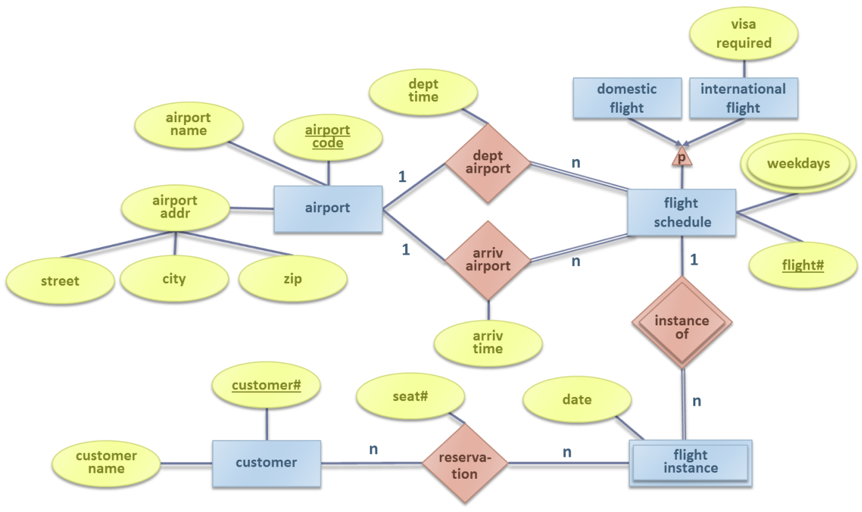
\includegraphics[width=\linewidth]{entities.png}
  \caption{Διάγραμμα Οντοτήτων/Συσχετίσεων}
\end{figure}


%%% Local Variables:
%%% mode: latex
%%% TeX-master: "main"
%%% End:
